% !TEX root = ../main.tex

%==========================================
\section{Problem Formulation}
\label{sec:problem}
%=========`=================================

%\san{Problem formulation could also be Experimental Setup / General comment: to be useful, this section needs to be intuitive from a human communication point of view. This is what motivates our pipeline and comparisons}

\note{1 column max; sections 1-4 must fit within the first 4 pages of the paper}\\
\note{Ece}


\begin{figure*}[t]
	\centering
	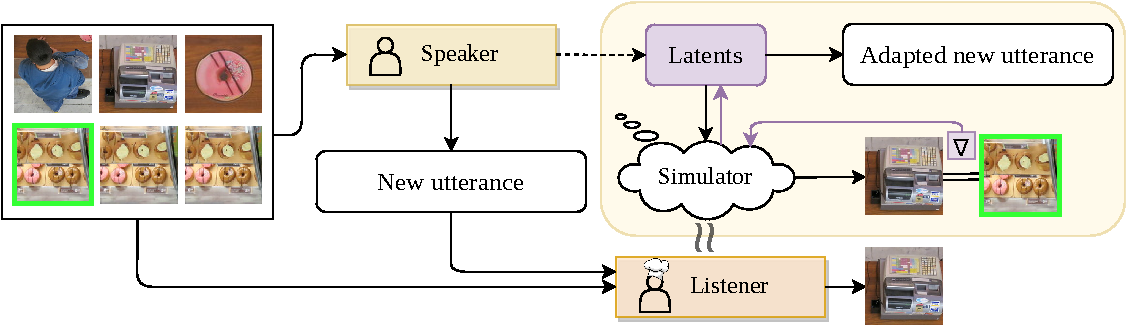
\includegraphics[width=2\columnwidth]{images/adaptation.pdf} %\hfill
	\caption{Adaptive pipeline \ece{images and utterances to be replaced with actual data} \san{Nice diagram! I'm not sure I fully understand the visual input, though: why are there 3 images that are the same?}\ece{just placeholders until we have actual outputs from adaptive speaker}} %\san{we could add two heads or robots to indicate that the generic speaker and the listener are two agents, while the domain-specific simulator is an idea (a bulb, a cloud?)} \mar{Should the purple arrow go from the simulator to the latents?}}
	\label{fig:pipeline}
\end{figure*}


%The different setups we compare (abstracting away from the specific models we use to implement them), including a diagram. What are the baselines / which ablations we consider, etc.

In our experimental setting, a speaker and a domain-specific listener play a referential game over a visual context in an asymmetric setup. That is, the listener lacks visual and linguistic information about domains other than its own area of expertise (e.g., \emph{food}).
In such cases, speakers may need to adapt their utterances to align with the domain of the listeners with the aim of achieving communicative success. %accommodate the listener's comprehension capacity with the aim of succeeding in game. In this work, we
%\san{In our experimental setting, a generic speaker and a domain-specific listener (e.g., a listener that only knows about \emph{food}) play a referential game over a visual context. To achieve communicative success, the speaker needs to adapt to the language domain of the listener. Since only the speaker adapts to the listener, the communicative setup is asymmetric. We} 
We model this behavior in our \textit{adaptive pipeline}. We have one listener per domain that we pair with the speaker in the game. Initially, the speaker produces an utterance for a target image among distractors based on its knowledge encompassing all the domains. However, to be successful, it then needs to adapt to the domain of the listener it is paired with, as the reference resolution performance of the listener is constrained by its domain-specific capabilities.

%We create this setting via first exposing the listeners only to \textit{domain-specific subsets} of the full dataset, which is used in training the speaker. The speaker learns to generate an utterance describing the target image from a point of view that encompasses all the domains. The aim of the listener is to predict the target image based on the speaker's utterance, albeit constrained by its own domain-specific capabilities. Via simulating the possible behavior of the listener, the speaker can alter its utterance on-the-fly. \san{All the above can be sign shortened: We have one listener per domain that we pair with the generic speaker in the game. Initially, the speaker utters a generic utterance, but then needs to adapt to the language of the listeners to be successful.}

\noindent\textbf{Adaptive pipeline} %\san{In human communication, a speaker can form their own idea of the listener as the interaction progresses. Inspired by this idea,}
In human communication, a speaker can form their own idea of the listener as the interaction progresses, and adapt their utterances accordingly. Inspired by this idea, in this pipeline, the speaker is endowed with the ability to adapt to the listener's knowledge space with the help of a domain-specific listener `simulator' (see Fig.~\ref{fig:pipeline}).  As the speaker would not have direct access to the internal states of the listeners, it can only use external indicators to guide its utterances: behavioral data coming from the listeners, i.e. listeners' predictions. In this way, the speaker is enhanced with a capacity for ToM and the ability to update its utterances by considering the listener's possible actions. Inspired by the PPLM method~\cite{dathathri2020plug}, \san{are we really getting inspired by this specific method or, more generally, by any CTG method that keep the LM parameters unaltered and operates at the decoding stage? If so, there are a couple more papers we could cite here} we implement an adaptation scheme in which the adaptation is effective only during an exchange with a single listener. In this way, the speaker can retain its domain-general capabilities. We compare the adaptive pipeline against one with a random listener (random), a non-adaptive speaker (baseline), and a domain-specific speaker (ceiling).

% \noindent\textbf{Baselines} 
% \san{The adaptive speaker is compared against a random speaker (random), a non-adaptive speaker (baseline), and domain-specific speaker (ceiling)}
% We compare the adaptive pipeline to 2 baselines: (1) random baseline (1-out-of-6, 16.67\%) and (2) the non-adaptive pipeline with the speaker and the domain-specific listeners, which would be our stronger baseline. As the ceiling, we evaluate domain-specific speakers that would generate utterances more aligned within a given domain without the need for on-the-fly adaptation.


% In this version of our pipeline, we first train a general speaker and a general listener independently. These general agents would be equipped with knowledge coming from all domains. In addition, using the domain-specific data, we train domain-specific listeners that are only exposed to the visual and linguistic concepts existing within the domain. After the training stage, the speaker and the listeners do not learn (i.e. they are frozen). 
% \ece{also pretraining a general listener using \textbf{generated} data from speaker or just evaluating it?} We store the utterances generated by the best speaker, the corresponding latents and the listeners' behavior given these utterances for the adaptive pipeline.
% 